% sections/00_introduction.tex: generated by newdeck/html2beamer.py from the HTML deck, then edited by hand

% ---------------------------------------------------------------- slide 2: Outline
\begin{btframe}{}{Outline}
\begin{outlinelist}
\outlineitem{1}{Introduction}{the background types, the geometry, the input muons and neutrinos}{1.00}
\outlineitem{2}{Simulation}{transport with Cuda Muons, inelastic scattering, hits and digitisation, trajectories}{1.00}
\outlineitem{3}{Selection}{track cuts, pair cuts (charge, DOCA, vertex, IP), time coincidence}{1.00}
\outlineitem{4}{Backgrounds before tagging}{muon and neutrino inelastic scattering, MS7 K\textsubscript{L}, combinatorial pairs}{1.00}
\outlineitem{5}{Background tagging}{reference designs R1, R2, R3}{1.00}
\outlineitem{6}{Optimisation and conclusion}{genetic-algorithm search, the optimised designs Z2 and Z3}{1.00}
\end{outlinelist}
\end{btframe}

% ---------------------------------------------------------------- slide 3: Four ways to fake a signal vertex in the decay volume
\begin{btframe}{1 · Introduction · the backgrounds}{Four ways to fake a signal vertex in the decay volume}
\noindent \begin{minipage}[t]{\dimexpr(0.5000\linewidth-0.5000\dimexpr11.49pt\relax)}\vspace{0pt}\raggedright
{\color{purple}\rule{\linewidth}{0.85pt}}\par\vspace{1.14pt}{\fontsize{5.23pt}{7.07pt}\selectfont \textcolor{purple}{\textbf{μ inelastic in MS7 → K\textsubscript{L}}}\par}
\vspace{0.41pt}
{\centering 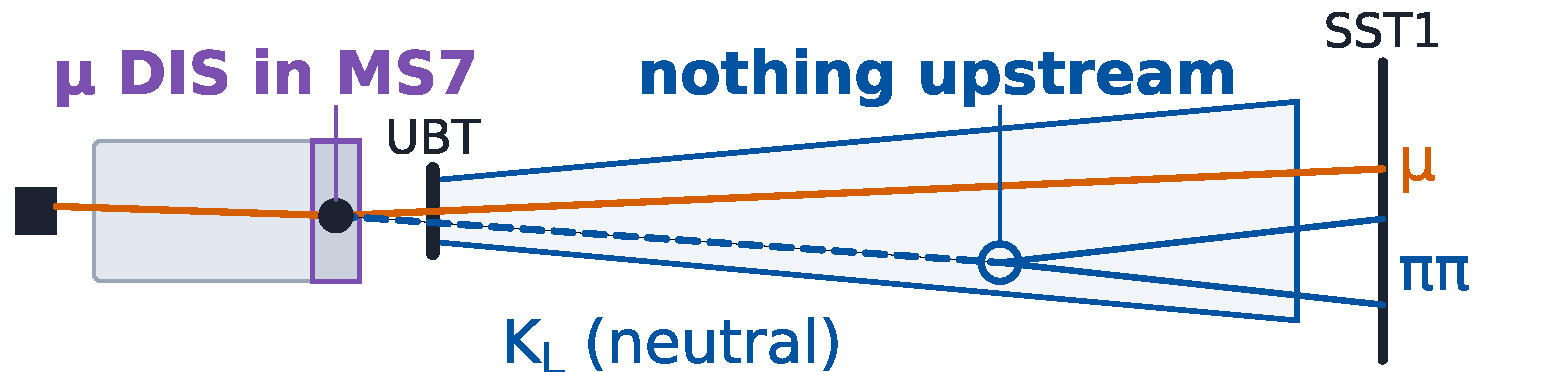
\includegraphics[width=1.00\linewidth,height=28.22pt,keepaspectratio]{figs/s02_sk1.pdf}\par}
\vspace{0.41pt}
{\fontsize{4.55pt}{6.15pt}\selectfont neutral: a K\textsubscript{L} made in the last iron of the shield decays in the vessel; nothing crosses the entrance\par}
\end{minipage}%
\hfill%
\begin{minipage}[t]{\dimexpr(0.5000\linewidth-0.5000\dimexpr11.49pt\relax)}\vspace{0pt}\raggedright
{\color{orange}\rule{\linewidth}{0.85pt}}\par\vspace{1.14pt}{\fontsize{5.23pt}{7.07pt}\selectfont \textcolor{orange}{\textbf{μ inelastic in the vessel}}\par}
\vspace{0.41pt}
{\centering 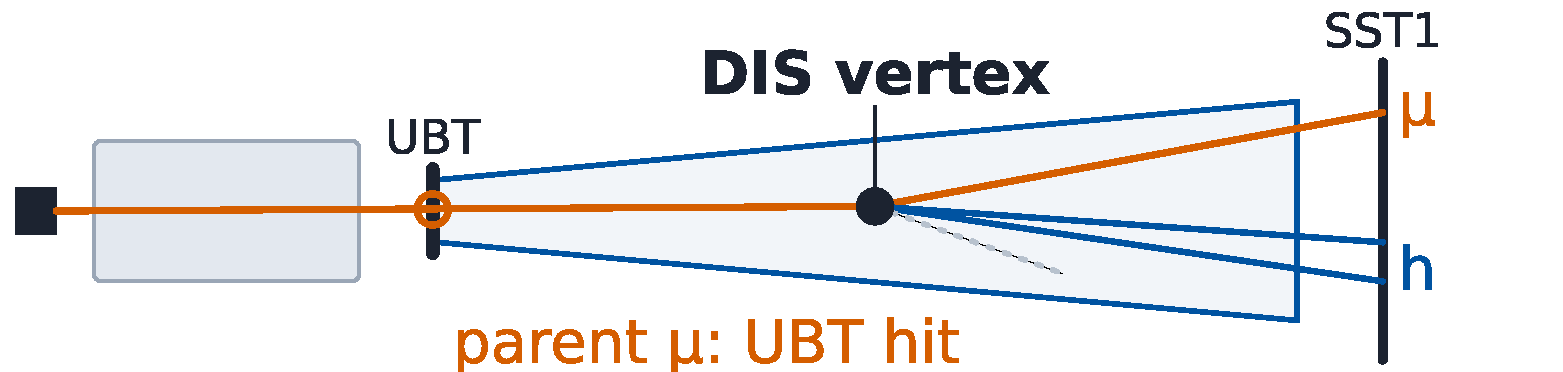
\includegraphics[width=1.00\linewidth,height=28.22pt,keepaspectratio]{figs/s02_sk2.pdf}\par}
\vspace{0.41pt}
{\fontsize{4.55pt}{6.15pt}\selectfont a real vertex in the helium or the walls; the parent muon crossed a tagger\par}
\end{minipage}\par
\vspace{1.37pt}
\noindent \begin{minipage}[t]{\dimexpr(0.5000\linewidth-0.5000\dimexpr11.49pt\relax)}\vspace{0pt}\raggedright
{\color{green}\rule{\linewidth}{0.85pt}}\par\vspace{1.14pt}{\fontsize{5.23pt}{7.07pt}\selectfont \textcolor{green}{\textbf{ν inelastic in the vessel and MS7}}\par}
\vspace{0.41pt}
{\centering 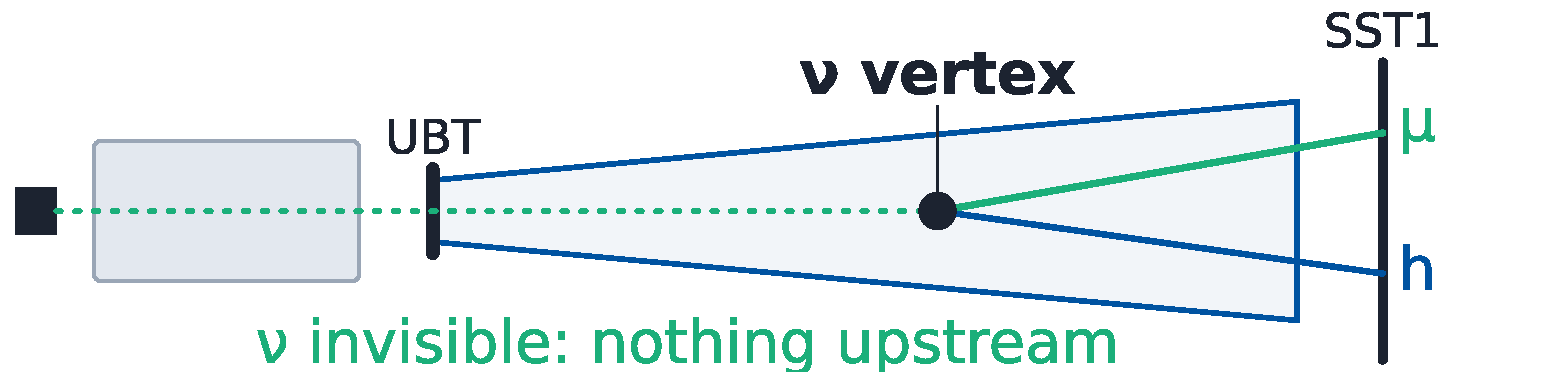
\includegraphics[width=1.00\linewidth,height=28.22pt,keepaspectratio]{figs/s02_sk3.pdf}\par}
\vspace{0.41pt}
{\fontsize{4.55pt}{6.15pt}\selectfont no incoming charged particle\par}
\end{minipage}%
\hfill%
\begin{minipage}[t]{\dimexpr(0.5000\linewidth-0.5000\dimexpr11.49pt\relax)}\vspace{0pt}\raggedright
{\color{cern}\rule{\linewidth}{0.85pt}}\par\vspace{1.14pt}{\fontsize{5.23pt}{7.07pt}\selectfont \textcolor{cern}{\textbf{combinatorial: μ × μ}}\par}
\vspace{0.41pt}
{\centering 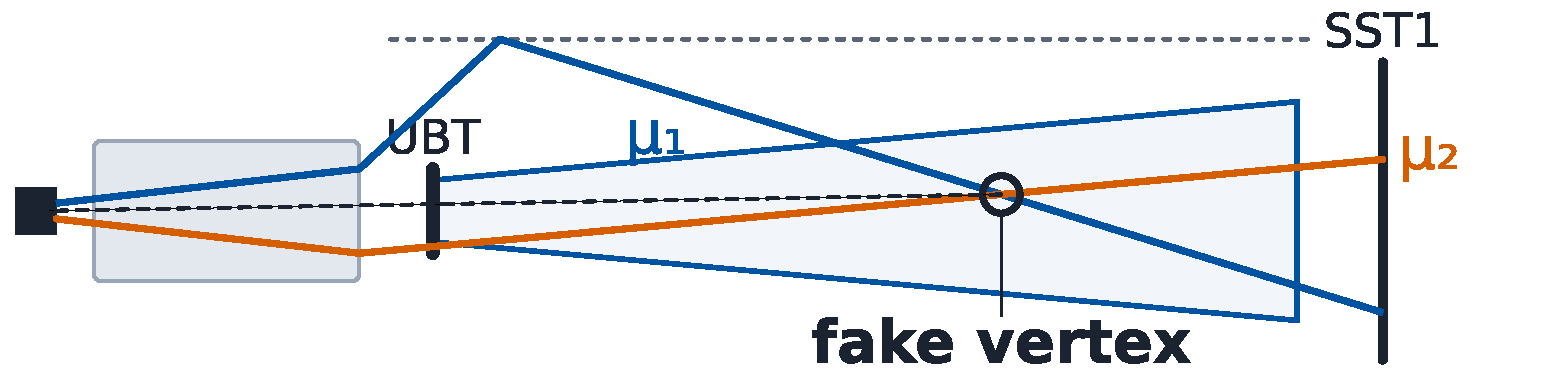
\includegraphics[width=1.00\linewidth,height=28.22pt,keepaspectratio]{figs/s02_sk4.pdf}\par}
\vspace{0.41pt}
{\fontsize{4.55pt}{6.15pt}\selectfont two muons from the target, in time by chance\par}
\end{minipage}\par
\vspace{1.37pt}
\noindent \begin{minipage}[t]{\dimexpr(0.5000\linewidth-0.5000\dimexpr11.49pt\relax)}\vspace{0pt}\raggedright
{\color{cern}\rule{\linewidth}{0.85pt}}\par\vspace{1.14pt}{\fontsize{5.23pt}{7.07pt}\selectfont \textcolor{cern}{\textbf{combinatorial: μ × interaction product}}\par}
\vspace{0.41pt}
{\centering 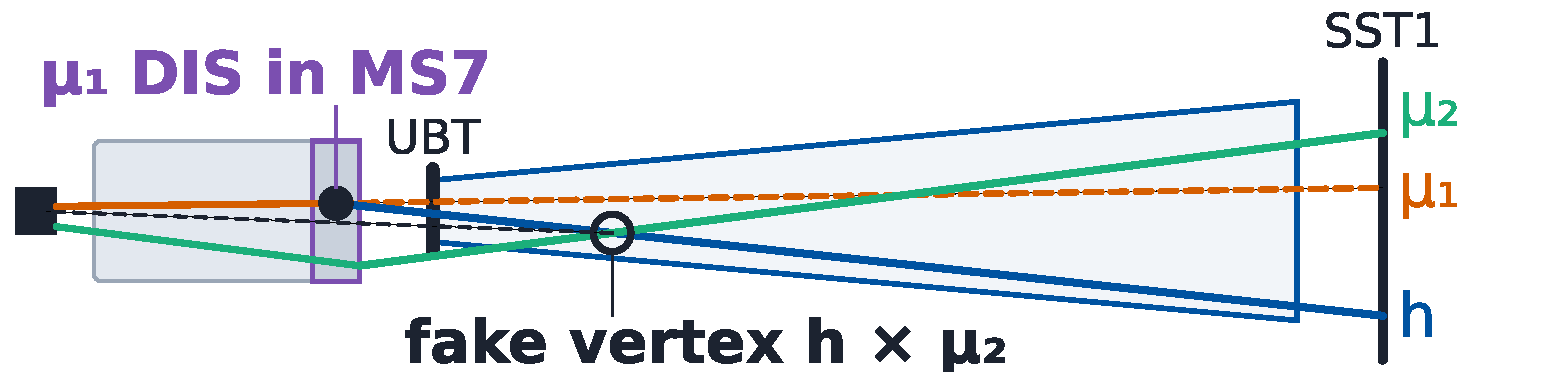
\includegraphics[width=1.00\linewidth,height=28.22pt,keepaspectratio]{figs/s02_sk5.pdf}\par}
\vspace{0.41pt}
{\fontsize{4.55pt}{6.15pt}\selectfont a muon with a charged product of an unrelated DIS (MS7, vessel)\par}
\end{minipage}%
\hfill%
\begin{minipage}[t]{\dimexpr(0.5000\linewidth-0.5000\dimexpr11.49pt\relax)}\vspace{0pt}\raggedright
{\color{cern}\rule{\linewidth}{0.85pt}}\par\vspace{1.14pt}{\fontsize{5.23pt}{7.07pt}\selectfont \textcolor{cern}{\textbf{combinatorial: μ × cavern-rock particle}}\par}
\vspace{0.41pt}
{\centering 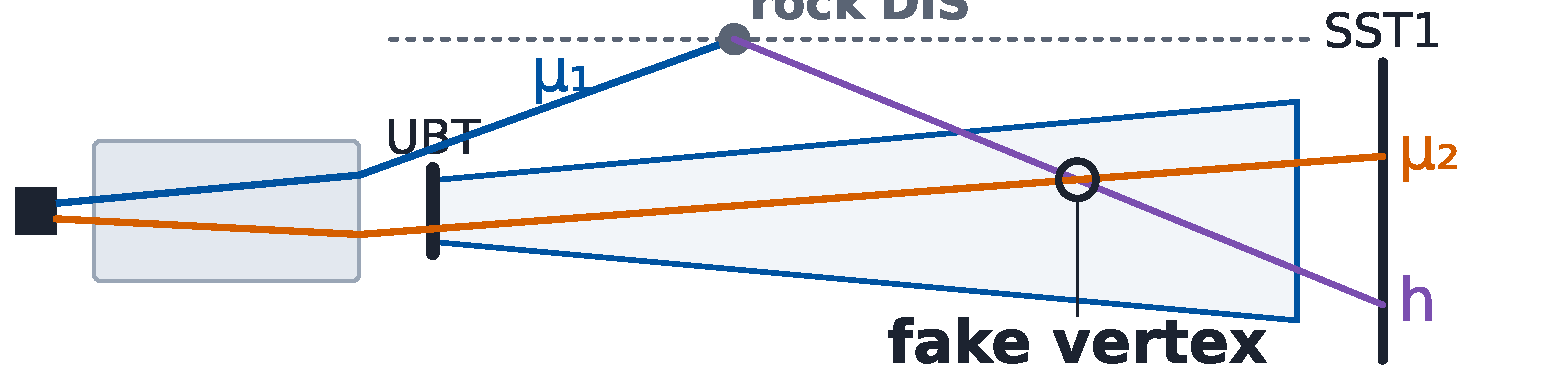
\includegraphics[width=1.00\linewidth,height=28.22pt,keepaspectratio]{figs/s02_sk6.pdf}\par}
\vspace{0.41pt}
{\fontsize{4.55pt}{6.15pt}\selectfont a muon with a hadron or electron from a muon interaction in the cavern rock\par}
\end{minipage}\par
\vspace{2.46pt}
{\fontsize{10.92pt}{14.99pt}\selectfont Inelastic = deep-inelastic and lower-energy muon–nucleus and ν–nucleus interactions. \\ Goal: \textbf{< 0.1 background events in 15 years} (6×10\textsuperscript{20} PoT).\par}
\end{btframe}

% ---------------------------------------------------------------- slide 4: Geometry in the simulation: FairShip 2026 layout
\begin{btframe}{1 · Introduction · geometry}{Geometry in the simulation: FairShip 2026 layout}
{\centering 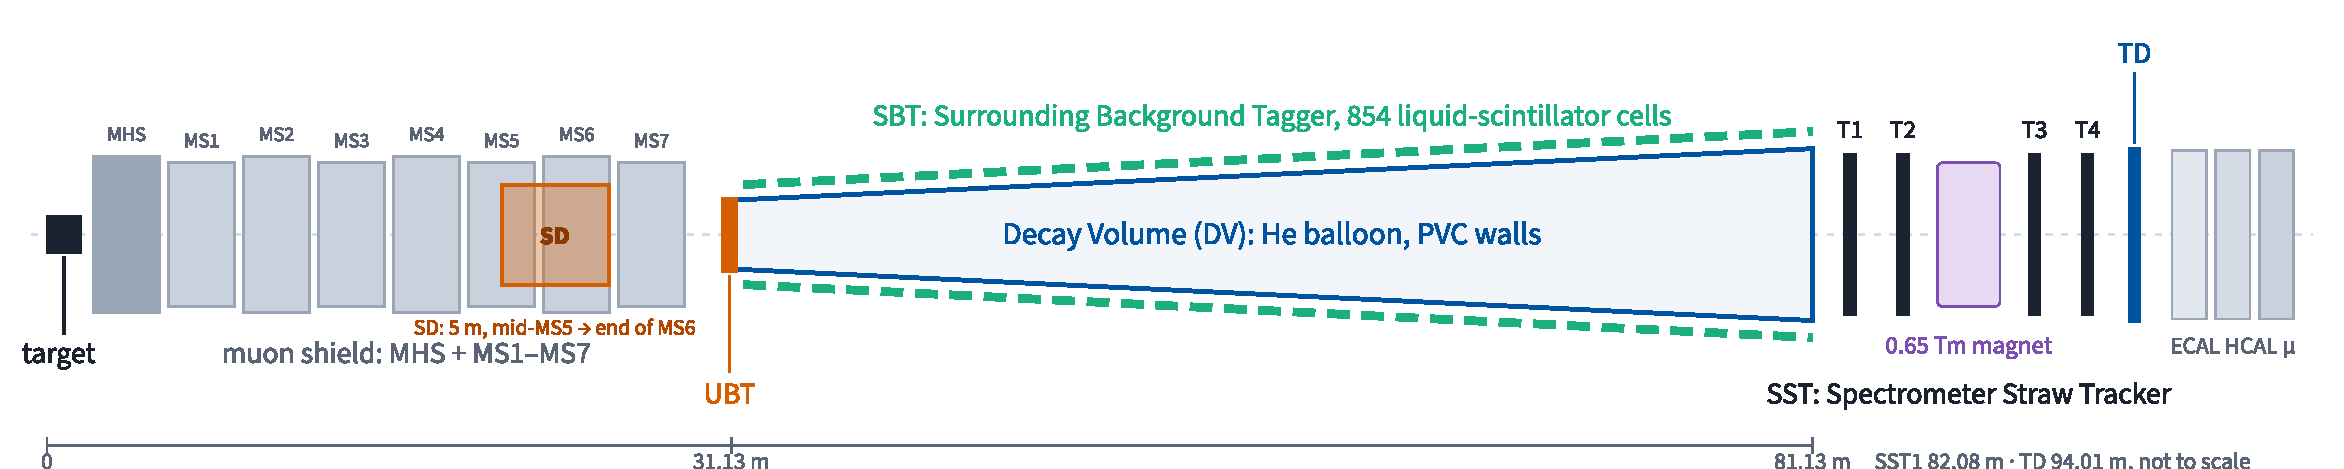
\includegraphics[width=1.00\linewidth,height=72.83pt,keepaspectratio]{figs/s03_sk1.pdf}\par}
\vspace{2.73pt}
{\fontsize{5.02pt}{6.52pt}\selectfont\setlength{\tabcolsep}{3.51pt}\renewcommand{\arraystretch}{1.42}
\begin{tabularx}{\linewidth}{l>{\raggedright\arraybackslash}Xl}
\textcolor{muted}{name} & \textcolor{muted}{what it is} & \textcolor{muted}{where} \\\headrule
MS & muon shield: MHS + MS1–MS7; MS7 = last magnet, iron z = 29.39–29.89 m & TRY6 (Nov-4 production) \\\rowrule
UBT & Upstream Background Tagger on the entrance window: vertical straws (1 × 2.7 m\textsuperscript{2}) + 4 × 4 m\textsuperscript{2} tile plane & z = 30.73 m (straws), 31.13 m (tiles) \\\rowrule
SBT & Surrounding Background Tagger: 20 cm liquid scintillator between 8 mm Al walls, 61 rings × 14 cells & z = 31.13 – 81.13 m \\\rowrule
DV & Decay Volume: frustum 1.0 × 2.7 m\textsuperscript{2} → 4 × 6 m\textsuperscript{2}, helium at 1 bar & z = 31.13 – 81.13 m \\\rowrule
SST, TD & spectrometer straw tracker (SST1 first station) and timing detector & SST1 82.08 m, TD 94.01 m \\\rowrule
MSMS & Muon Shield Monitoring System: silicon strip stations inside the MS7 iron (R3) & z = 29.39, 29.59, 29.79 m \\\rowrule
\end{tabularx}\par}
\slidenote{Names: CERN-SHiP-INT-2025-004 (Note\_combinatorial\_background, sec. 1, 3.1, 5). Source: veto lib/veto/geometry.py (FairShip geometry\_config 2026-0.1, target-aligned z = z\textsubscript{FS} − 2.14 m)}
\end{btframe}

% ---------------------------------------------------------------- slide 5: Initial sample: muons and neutrinos from the target
\begin{btframe}{1 · Introduction · the input}{Initial sample: muons and neutrinos from the target}
{\fontsize{4.55pt}{5.92pt}\selectfont\setlength{\tabcolsep}{3.19pt}\renewcommand{\arraystretch}{1.42}
\begin{tabularx}{\linewidth}{lrr>{\raggedright\arraybackslash}X>{\raggedright\arraybackslash}X}
\textcolor{muted}{sample} & \textcolor{muted}{source} & \textcolor{muted}{per spill (4×10\textsuperscript{13} PoT; stat. < 1 \%)} & \textcolor{muted}{transport} & \textcolor{muted}{stored / cuts} \\\headrule
muons & Nov-4 target pool (Shah Rukh, Nov 2026) & 4.70×10\textsuperscript{10} (μ\textsuperscript{+} 2.5×10\textsuperscript{10}, μ\textsuperscript{-} 2.2×10\textsuperscript{10}) & Cuda Muons through TRY6 + TCC8 rock + cavern, 3 220 seeds = 3 220 spills & states at z = 30.6 m and at SST1 (shell storage, 7.7×10\textsuperscript{8} rows) \\\rowrule
neutrinos & 2026 production (target + shield) & 4.2×10\textsuperscript{11} (ν\textsubscript{μ} 2.2×10\textsuperscript{11}, ν̄\textsubscript{μ} 1.6×10\textsuperscript{11}, ν\textsubscript{e} + ν̄\textsubscript{e} 4.3×10\textsuperscript{10}, ν\textsubscript{τ} + ν̄\textsubscript{τ} 3×10\textsuperscript{9}) & straight lines; GENIE 3.06 interactions forced in every target & E > 1 GeV, θ < 0.3 rad \\\rowrule
\end{tabularx}\par}
\vspace{2.46pt}
\noindent \begin{minipage}[t]{\dimexpr(0.5745\linewidth-0.5745\dimexpr9.67pt\relax)}\vspace{0pt}\raggedright
{\centering 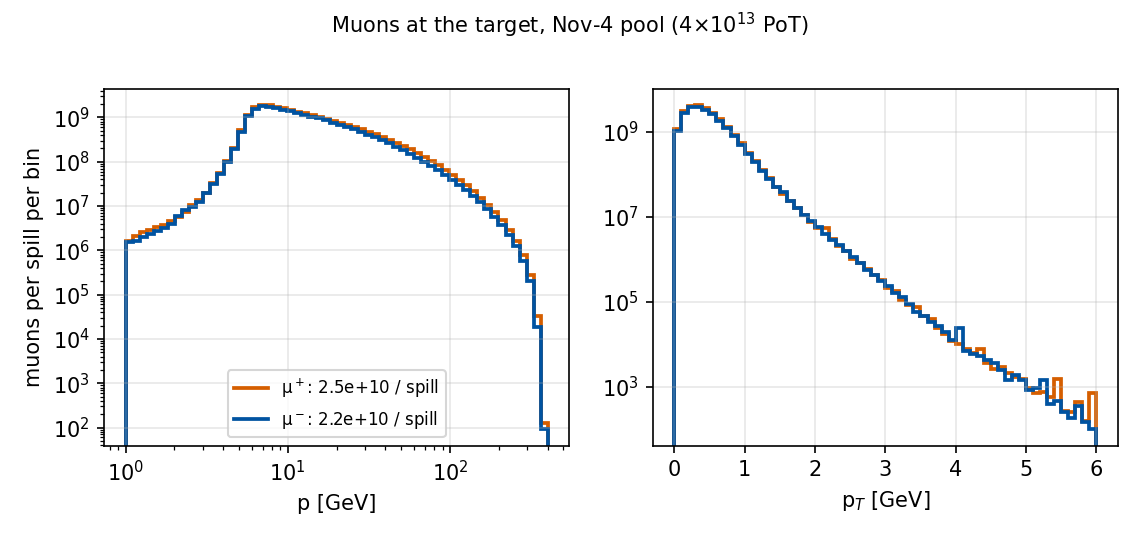
\includegraphics[width=1.00\linewidth,keepaspectratio]{figs/s04_img1.png}\par}
\end{minipage}%
\hfill%
\begin{minipage}[t]{\dimexpr(0.4255\linewidth-0.4255\dimexpr9.67pt\relax)}\vspace{0pt}\raggedright
{\centering 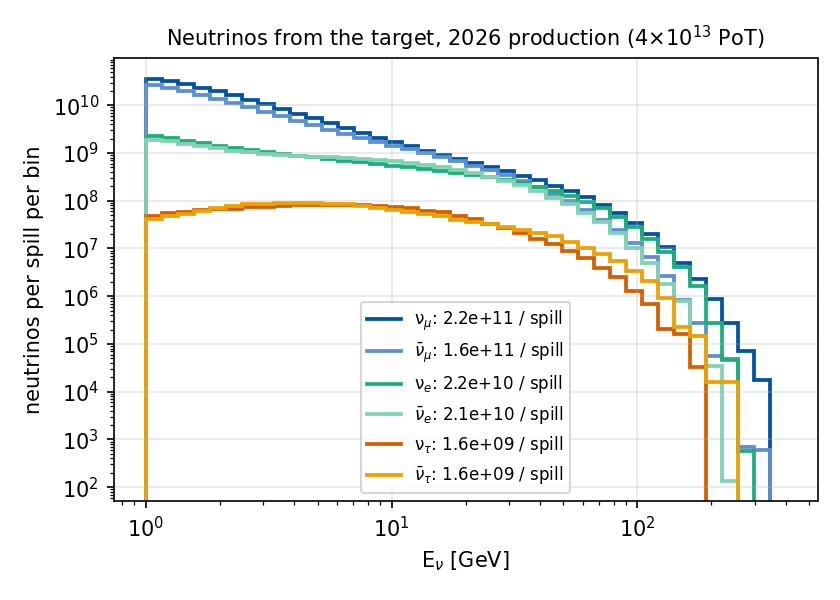
\includegraphics[width=1.00\linewidth,keepaspectratio]{figs/s04_img2.png}\par}
\end{minipage}\par
\vspace{2.46pt}
{\fontsize{6.02pt}{8.43pt}\selectfont
\begin{itemize}
  \item \textbf{Nov-4 production} (Shah Rukh), used for every number in this talk; one seed = the whole pool once = one spill of 4×10\textsuperscript{13} PoT; 15 years = 1.5×10\textsuperscript{7} spills
\end{itemize}}
\end{btframe}
